\section{Einleitung}
Diese Dokument stellt die Dokumentation des Projekts \emph{Raspberry PI Security Application}, in weiterer Folge \emph{RPISec} genannt, dar, das für die Lehrveranstaltung \emph{Mobile und ubiquitäre Systeme} realisiert wurde. In diesem Projekt wurde eine Heimsicherheitsanwendung mit Raspberry PI, Docker und Spring realisiert, die bei einem Sicherheitsverstoß in der Lage ist, bekannte mobile Endgeräte von registrierten Benutzern über diesen Sicherheitsverstoß zu informieren. 

\subsection{Problemdarstellung}
Dieser Abschnitt behandelt die Problemdarstellung, welche die Grundlage für die zu implementierende \emph{Raspberry PI Security Application} ist. Bei einem Auslösen eines Bewegungssensors in einem Haushalt sollen alle Bewohner über ihre mobilen Endgeräte wie Handy und Tablet über den Vorfall informiert werden sowie ein Foto erhalten, das den Sicherheitsbereich, zum Zeitpunkt wann der Bewegungsmelder ausgelöst wurde, zeigt. Des weiteren soll es zu jedem Zeitpunkt möglich sein sich ein aktuelles Foto des Sicherheitsbereichs über ein mobiles Endgerät zu beziehen.  
\newline
\newline
Da es sich um eine Sicherheitsanwendung handelt, soll die Benutzerverwaltung sowie die Authentifizierung \emph{In-House} gehalten werden, also die Sicherheitsanwendung selbst soll in der Lage sein die Benutzer zu verwalten und die Authentifizierungen durchzuführen. Da sich die mobilen Endgeräte in irgendwelchen Netzen ans Internet anbinden können, wie zum Beispiel über einen Mobilfunkanbieter, Internetanbieter oder öffentlichen \emph{Hot-Spot}, wird ein \emph{Messaging} Dienst benötigt über den die mobilen Endgeräte erreicht werden können. Dieser muss es erlauben, dass die Benutzerverwaltung von einem anderen Dienst übernommen werden kann, da wir diesen \emph{Messaging} Dienst nicht vertrauen wollen und daher den \emph{Messaging} Dienst auch nicht die Benutzerverwaltung überlassen wollen.


\subsection{Funktionsweise}
Dieser Abschnitt behandelt die Funktionsweise der Applikation \emph{RPISec}. Die Abbildung \ref{fig:image-system-structure} zeigt den Systemaufbau der \emph{RPISec} Applikation. 
\begin{figure}[h]
	\centering
	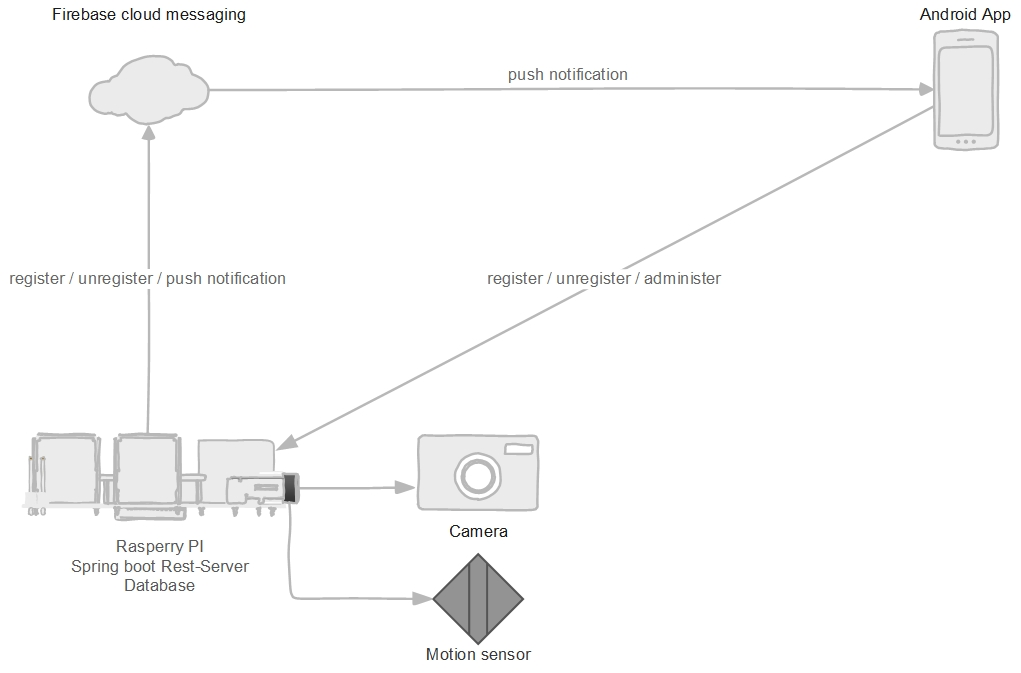
\includegraphics[scale=0.7]{\imageDir/Infrastructure.jpg}
	\caption{Systemaufbau der \emph{RPISec} Applikation}
	\label{fig:image-system-structure}
\end{figure}
\ \newpage

\subsubsection{Zugangsbestätigung eines neuen Benutzers}
Beim Start des \emph{Auth-Service} wird ein Administrator Benutzer erstellt, der über eine E-Mail dazu aufgefordert wird, seinen Zugang zu aktivieren, in dem er ein Password für den Benutzer vergeben wird.
\begin{figure}[h]
	\centering
	
\includegraphics[scale=0.5]{\imageDir/view-verify-account.JPG}
	\caption{Zugangsaktivierung}
	\label{fig:image-veriy-account}
\end{figure}
\begin{figure}[h]
	\centering
	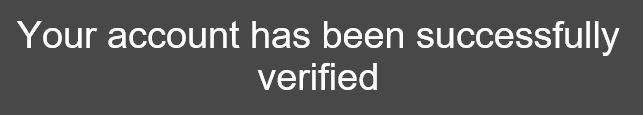
\includegraphics[scale=0.5]{\imageDir/view-verified-account.JPG}
	\caption{Bestätigung der Aktivierung}
	\label{fig:image-veriied-account}
\end{figure}
\subsubsection{\emph{Client Login}}
\begin{figure}[h]
	\centering
	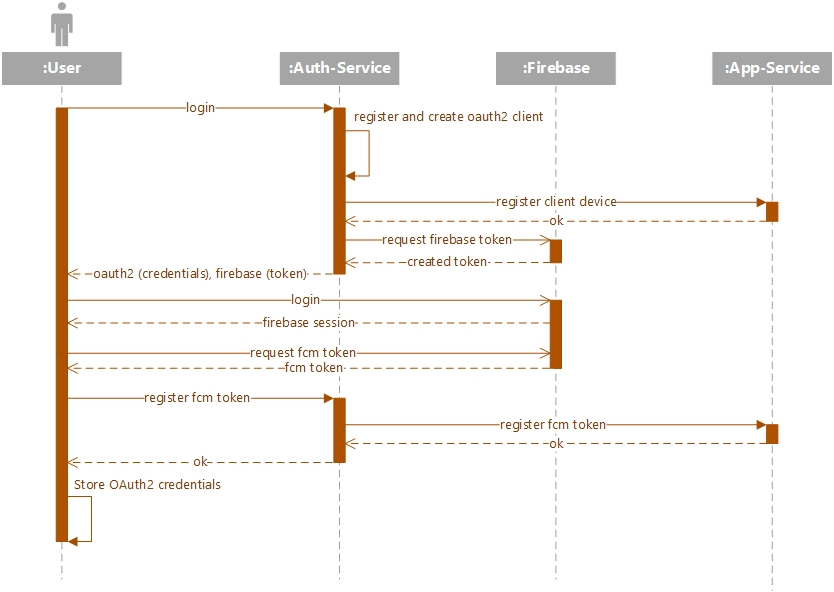
\includegraphics[scale=0.55]{\imageDir/sequence-client-login.jpg}
	\caption{Sequenzdiagramm des Logins über einen mobilen \emph{Client}}
	\label{fig:image-sequence-client-login}
\end{figure}
Die Abbildung \ref{fig:image-sequence-client-login} zeigt das Sequenzdiagramm das den erfolgreichen Ablauf des Logins eines Benutzers über ein Android Gerät beschreibt. Im Zuge des Logins wird das mobile Endgerät am Authentifizierungsservice und Applikationsservice registriert und für jeden Login ein neuer \emph{OAuth2 Client} angelegt und gegebenenfalls der alte \emph{OAuth2 Client} für dieses Endgerät gelöscht. Bezüglich OAuth2 wurde dieser Ansatz gewählt, da mit der \emph{Client}-Applikation keine \emph{Oauth2 Client} Zugangsdaten ausgeliefert sollen.

\subsubsection{Sicherheitsvorfall melden}
\begin{figure}[h]
	\centering
	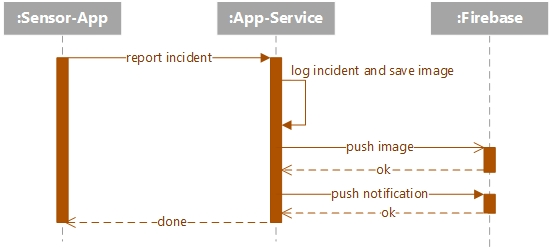
\includegraphics[scale=0.55]{\imageDir/sequence-incident.jpg}
	\caption{Sequenzdiagramm des Behandelns eines Sicherheitsvorfalls}
	\label{fig:image-sequence-incident}
\end{figure}
\ \newline
Die Abbildung \ref{fig:image-sequence-incident} zeigt das Sequenzdiagramm für das Behandeln eines Sicherheitsvorfalls, der von der Sensorapplikation erkannt und dem Applikationsservice mitgeteilt wurde. Der Vorfall wird über \emph{Firebase} an die \emph{Clients} gemeldet, wobei einerseits eine \emph{Cloud Message} an die \emph{Clients} versendet wird, sowie das gemachte Bild in der \emph{Firebase} JSON-Datenbank den \emph{Clients} zum Download zur Verfügung gestellt wird.  
 
\subsubsection{\emph{Client} Nachrichtenempfang}
\begin{figure}[h]
	\centering
	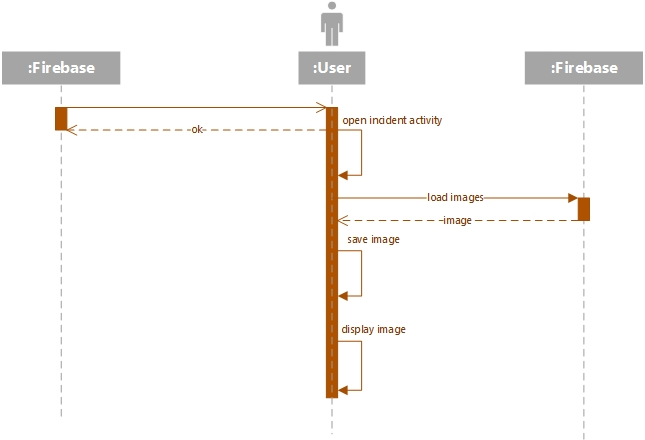
\includegraphics[scale=0.55]{\imageDir/sequence-client-notification.jpg}
	\caption{Sequenzdiagramm der Benachrichtigung eines \emph{Client}}
	\label{fig:image-sequence-client-notification}
\end{figure}
\ \newline
Die Abbildung \ref{fig:image-sequence-client-notification} zeigt den Ablauf einer  Benachrichtigung eines \emph{Client} über den \emph{Firebase Messaging} Dienst. Nachdem auf die Nachricht geklickt wurde, wird eine \emph{Activity} für das Anzeigen der Bilder geöffnet, die alle bereits gespeicherten Bilder und das neu geladene Bild anzeigt. 